\renewcommand{\prevpart}{0 }
\renewcommand{\thispart}{1 }
\renewcommand{\nextpart}{2 }

\section{Introduction to Machine Learning}

% Cover page
%
% Cover page for giveb part
%

\title[\modulename - Part \thispart]
{
  {\bf 
   \modulename - 
   Part \thispart\\
  }
  \vspace{0.5cm}
  {\it 
   \color{yellow}
    \secname\\
  }
}
\author[C.Andreopoulos] {
  Professor Costas Andreopoulos\inst{1,2}, {\it FHEA}
}
\institute[Liverpool/STFC-RAL] {
   \inst{1} University of Liverpool, Department of Physics\\
   \vspace{0.3cm}
   {\it {\color{magenta} Lectures delivered at the University of Liverpool, 2024-25}}\\
   \vspace{0.2cm}
}
\date{\today}

\titlegraphic{
  
\includegraphics[height=30px]{images/logo/liverpool.png}
}

\begin{frame}[plain]
  \titlepage
\end{frame}




% Outline
%
% Table of contents to be displayed at the beginning of each part
%

\begin{frame}[t,allowframebreaks]{Outline for Part \thispart -}
  % Part \thispart (\secname) covers the following topics:\\
  % \vspace{0.5cm}
  \linespread{1.1}
  \setcounter{secnumdepth}{3}
  \setcounter{tocdepth}{3}
  % \tableofcontents[currentsection, hideothersubsections, sectionstyle=hide/hide]
  \tableofcontents[part=\thispart]
\end{frame}



% %
% % Cover page
% %

% \title[\modulename - Part \thispart]
% { 
%   {\bf 
%    \modulename - 
%     Part \thispart\\
%   }
%   \vspace{0.5cm}
%   {\it 
%    \color{yellow}
%     Introduction to Machine Learning\\
%   }
% }

% \author[C.Andreopoulos] {
  Professor Costas Andreopoulos\inst{1,2}, {\it FHEA}
}
\institute[Liverpool/STFC-RAL] {
   \inst{1} University of Liverpool, Department of Physics\\
   \vspace{0.3cm}
   {\it {\color{magenta} Lectures delivered at the University of Liverpool, 2024-25}}\\
   \vspace{0.2cm}
}
\date{\today}

\titlegraphic{
  
\includegraphics[height=30px]{images/logo/liverpool.png}
}


% \begin{frame}[plain]
%   \titlepage
% \end{frame}

% % Plan 
% \begin{frame}[t,allowframebreaks]{Outline for Part \thispart -}
%   Part \thispart (\secname) covers the following topics:\\
%   \vspace{0.5cm}
%   \setcounter{tocdepth}{2}
%   \tableofcontents[currentsection, hideothersubsections, sectionstyle=hide/hide]
% \end{frame}
% %\begin{frame}{Plan for Part \thispart}


\end{frame}



% Precursors
\subsection{Precursors of artificial intelligence}


% History of AI
\subsection{History of artificial intelligence}
\subsubsection{Blah}
\subsubsection{Blah}
\subsubsection{Blah}
\subsubsection{Blah}
\subsubsection{Blah}
\subsubsection{Blah}
\begin{frame}{The history of AI\footnote{
\tiny For a detailed discussion, see \url{https://en.wikipedia.org/wiki/History_of_artificial_intelligence}}}

\begin{itemize}
\item Birth of AI (1952-1956)
\item Symbolic AI (1956-1974)
\item First AI winter (1974-1980)
\item Boom (1980-1987)
\item Bust: Second AI winter (1987-1993)
\item AI (1993-2011)
\item Deep learning, big data and AI (2011-present)

\end{itemize}

\end{frame}



\subsection{Human vs computer learning}

\subsection{Different learning paradigms: Supervised, unsupervised and reinforcement learning}

\subsection{Artificial intelligence, machine learning and deep learning}

\subsection{Machine learning tasks}

\subsection{A simple practical example: Linear regression}

\subsection{Biologically inspired methods of computer learning}

\subsection{Basic architecture of neural networks}

\subsection{Fundamental concepts}


% From AI to DL
\begin{frame}{Connection between AI, ML and DL}

\index{AI}\index{artificial intelligence}\gls{ai} -
\gls{ai}
\gls{ml}
\gls{dl}

    \begin{center}
        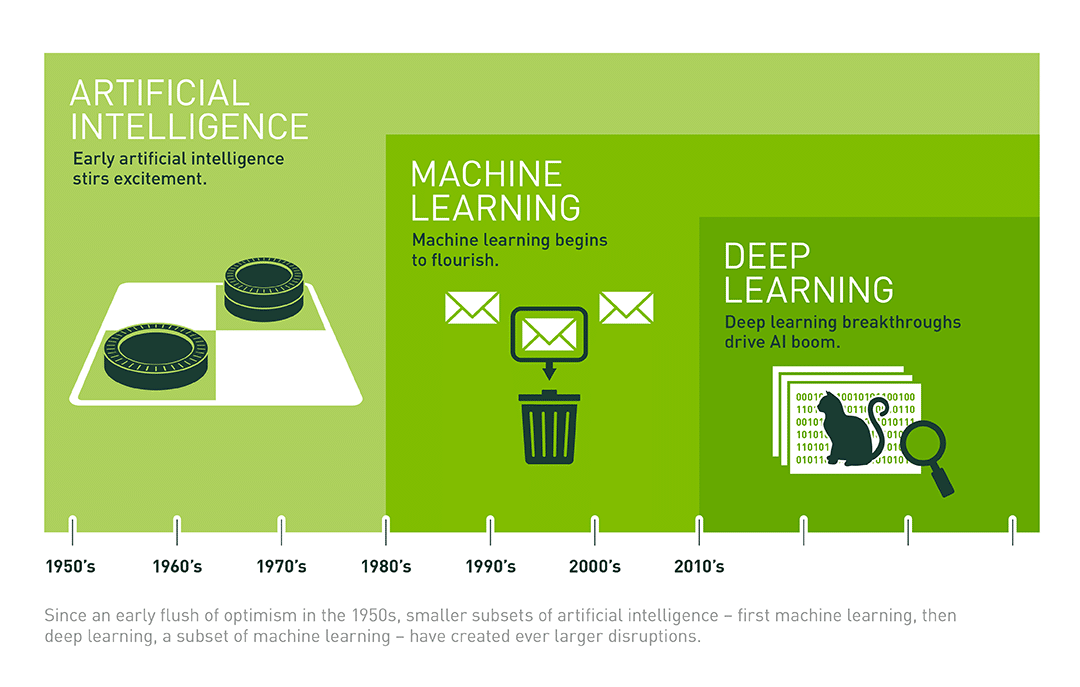
\includegraphics[width=0.90\textwidth]{./images/dl_intro/ai_ml_dl.png}\\
        {\scriptsize Image reproduced from \cite{NVidiaBlog:DifferenceBetweenAIMLDL}}\\
    \end{center}

\end{frame}
    


%---
\begin{frame}{Blah}

\end{frame}
%---

% Main points to remember
\renewcommand{\partsummarytitle}{Main points to remember }
\renewcommand{\summarizedlecture}{1 }

%
%
%

\begin{frame}{Lecture \summarizedlecture - \lecturesummarytitle}


\end{frame}



% Preview of next part
\begin{frame}{Preview of Lecture \nextlecture}

\begin{itemize}
{\small
\item blah
\item blah
}
\end{itemize}

\end{frame}



% References and suggested reading for this part
%
%
%

\begin{frame}{Suggested reading for Part \thispart}

    {
        \small
        Essential reading on {\bf automatic differentiation}:
        \begin{itemize}
            \scriptsize
            \item Section 6.5 from the `Deep Learning' 
            textbook of Goodfellow, Bengio and Courville \cite{Goodfellow:2017MITDL}.
            \item Appendix B from the `Machine Learning Refined' 
            textbook of Watt, Borhani and Katsaggelos \cite{Watt:2016Cambridge}.
            \item `A review of automatic differentiation and its 
            efficient implementation' by Margossian \cite{Margossian:2019ad}
        \end{itemize}
        
        Also, you may want to browse:
        \begin{itemize}
            \scriptsize
            \item The collection of articles
             in the book `Automatic Differentiation: Applications, Theory, and Implementations'
             edited by B{\"u}cker, Corliss, Hovland, Naumann and Norris \cite{Bucker:2005ABo}
        \end{itemize}
    }
    

\end{frame}

% Optional material


